\section{Systemidentifikation}
\subsection{Basics}
\begin{itemize}
	\item Gewinnen von Informationen über ein nur teilweises oder ganz unbekanntes System
	\item \textbf{Achtung:} Bei Bode-Diagramm ist X-Achse in $\omega$ und nicht in der Frequenz 
	\begin{itemize}
		\item Reminder: $x \left[db\right] = 20\log_{10}\left(x\right)$
	\end{itemize}
	\item Erstellen von mathematischen Modellen basierend auf den Messergebnissen
	\item 
\end{itemize}

\subsection{Nicht Parametrische Identifikation}
\begin{itemize}
	\item Anregung eines Systems mit dem Sinus einer einzelnen Frequenz und beobachten des Ausganges
	\item Beobachten der Antwort und entsprechende Erstellung des Bode-Diagramms
	\item Für eine Totzeit ($e^{-st_t}$) geht der Phasengang mit zunehmender Frequenz zu $-\infty$, der Amplitudengang wird nicht beeinflusst. 
\end{itemize}
\begin{figure}[h!]
	\centering
	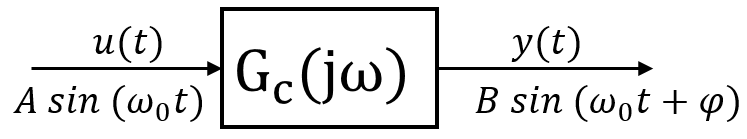
\includegraphics[width=0.25\linewidth]{bilder/sysIdent1}
\end{figure}

\subsubsection{Bode $\Leftrightarrow$ Übertragungsfunktion}
\begin{tabularx}{\linewidth}{p{0.25\linewidth} p{0.25\linewidth} p{0.25\linewidth} p{0.25\linewidth} }
	\textbf{Integrator} 	&\textbf{Tiefpass}			&\textbf{Hochpass}				&\textbf{Resonanz}	\\
	%Zeile 2 mit Allen Bildern
	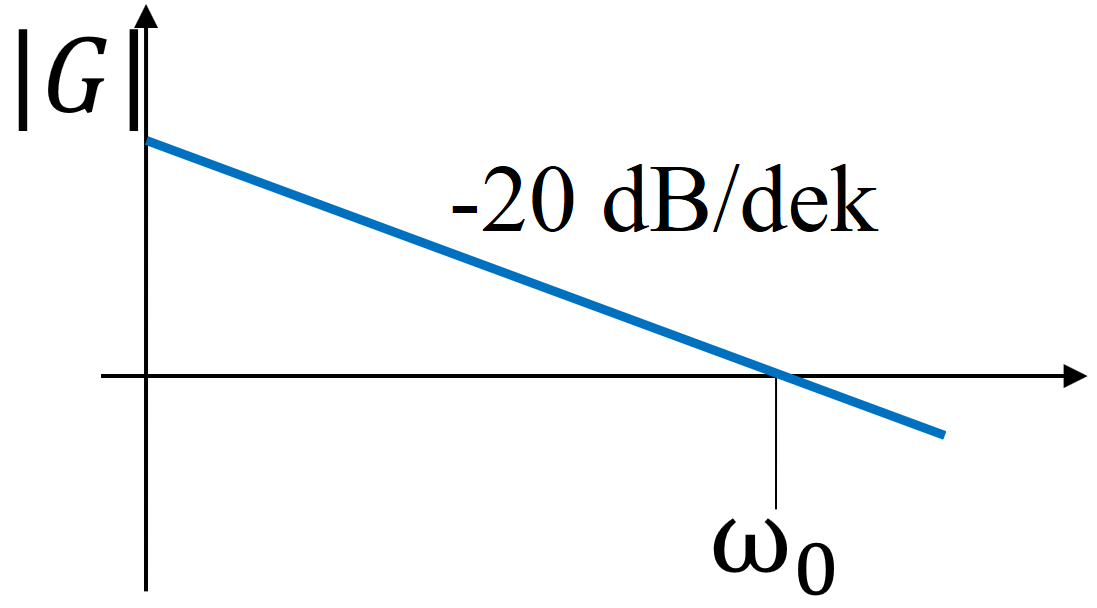
\includegraphics[width=.75\linewidth]{bilder/sysIdentInt}&
	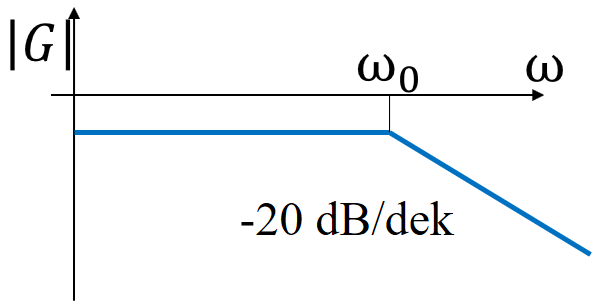
\includegraphics[width=.75\linewidth]{bilder/sysIdentTiefpass}&
	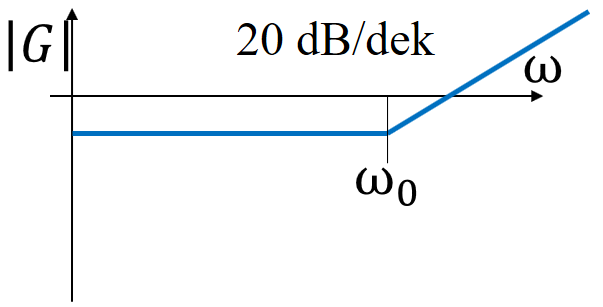
\includegraphics[width=.75\linewidth]{bilder/sysIdentHochpass}&
	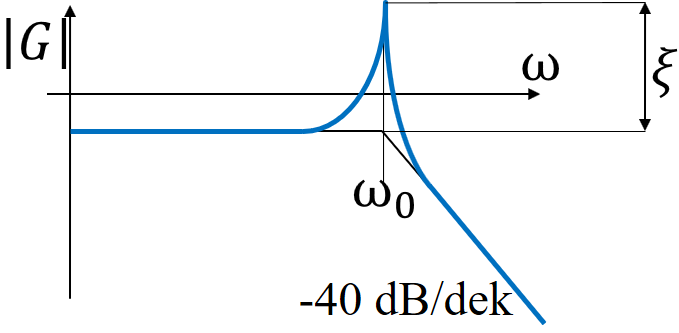
\includegraphics[width=.75\linewidth]{bilder/sysIdentResonanz}\\
	%Zeile 3 Mit den Formeln
	\begin{equation*}
		G\left(s\right) = \frac{\omega_0}{s}
	\end{equation*}&
	\begin{align*}
		G\left(s\right)= \frac{1}{\frac{1}{\omega_0}s+1}  \\
						=\frac{\omega_0}{s+\omega_0}
	\end{align*}&
	\begin{equation*}
		G\left(s\right)=\frac{1}{\omega_0}+1
	\end{equation*}&
	\begin{align*}
	\nonumber
		G\left(s\right) =\frac{1}{s^2T_0^2+2\xi T_0+1} \\
		T = \frac{2\pi}{\omega_0}
	\end{align*} 
\end{tabularx}

\subsubsection{Leakage-Effekt}
\begin{itemize}
	\item Zu erkennen wenn:
	\begin{itemize}
		\item Verstärkung zwischen $u(s)$ und $y(s)$ auf einmal fast konstant bei 0 dB bleibt 
		\item Das bekannte und gleichzeitig gemessene Eingangssignal $u(s)$ scheint bei zunehmender Frequenz gedämpft zu sein. 
		\item Ein untypischer Knick, der in dem Bode-Diagramm auftritt. Hierbei muss sichergestellt werden, dass dieser nicht aufgrund der Regelstrecke ist
	\end{itemize}
	\item In untenstehenden Grafiken sind Beispiele von Leakage-Effekten gezeigt. Die feine Linie ist dabei das wahre Verhalten des Systems, die dicke Linie das gemessene Verhalten des Systems.
\end{itemize}
\begin{figure}[!ht]
	\centering
	\subfloat[Gemessene Amplitude von $u(s)$ und $y(s)$ \label{subfig:Leakage1}]{
		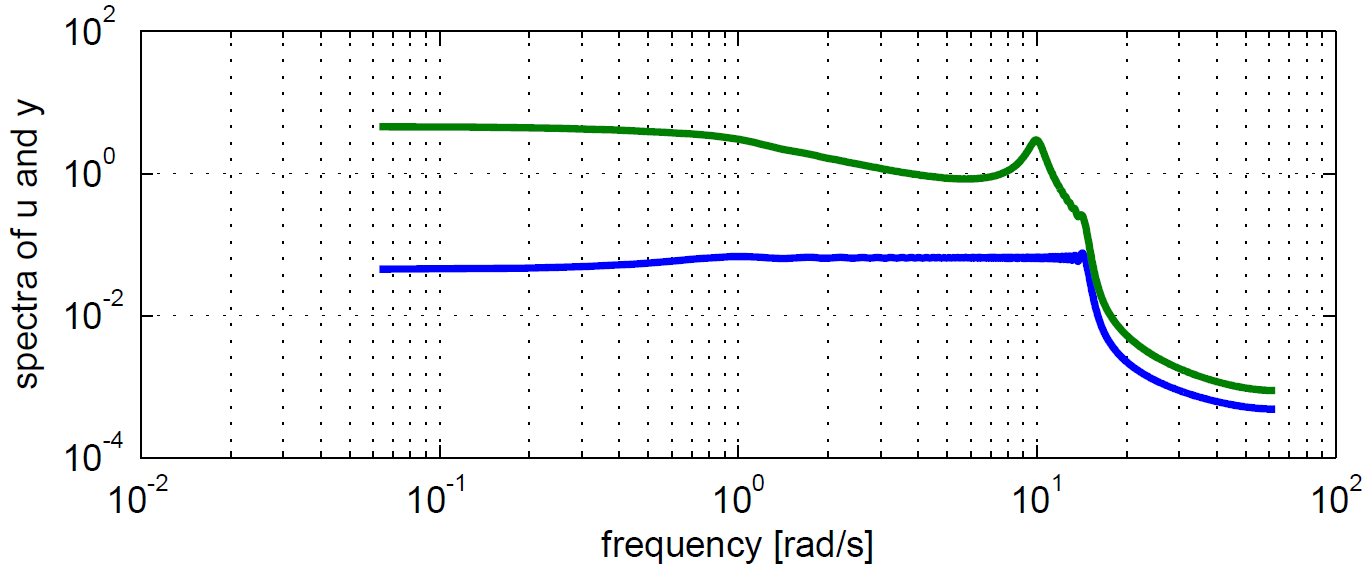
\includegraphics[width=0.3\textwidth]{./bilder/LeakageEffect1.PNG}
	}
	\subfloat[Amplitudengang der Regelstrecke \label{subfig:Leakage2}]{
		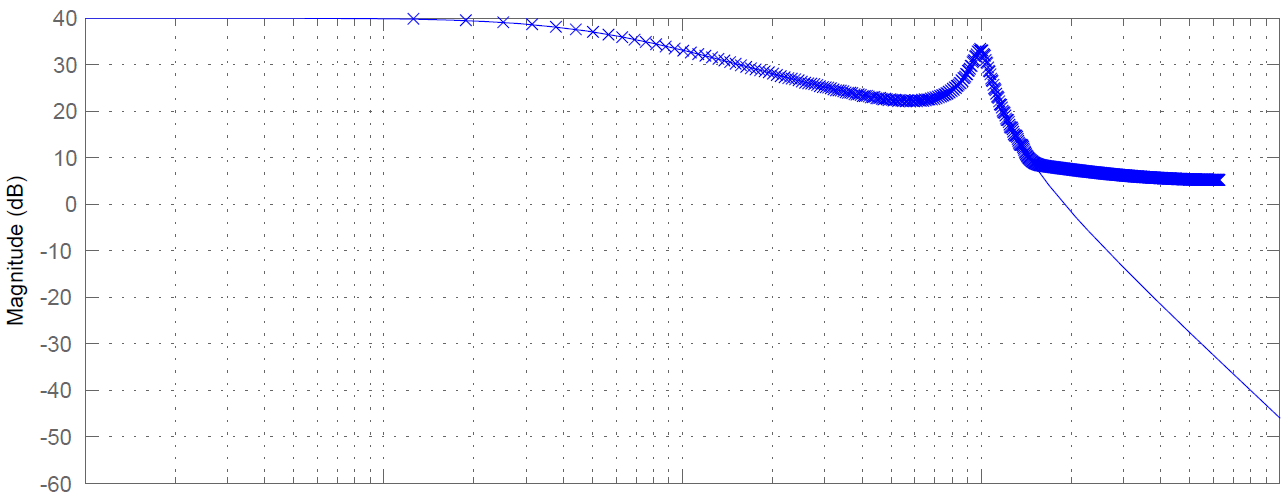
\includegraphics[width=0.3\textwidth]{./bilder/LeakageEffect2.PNG}
	}
	\subfloat[Phasengang der Regelstrecke \label{subfig:Leakage3}]{
		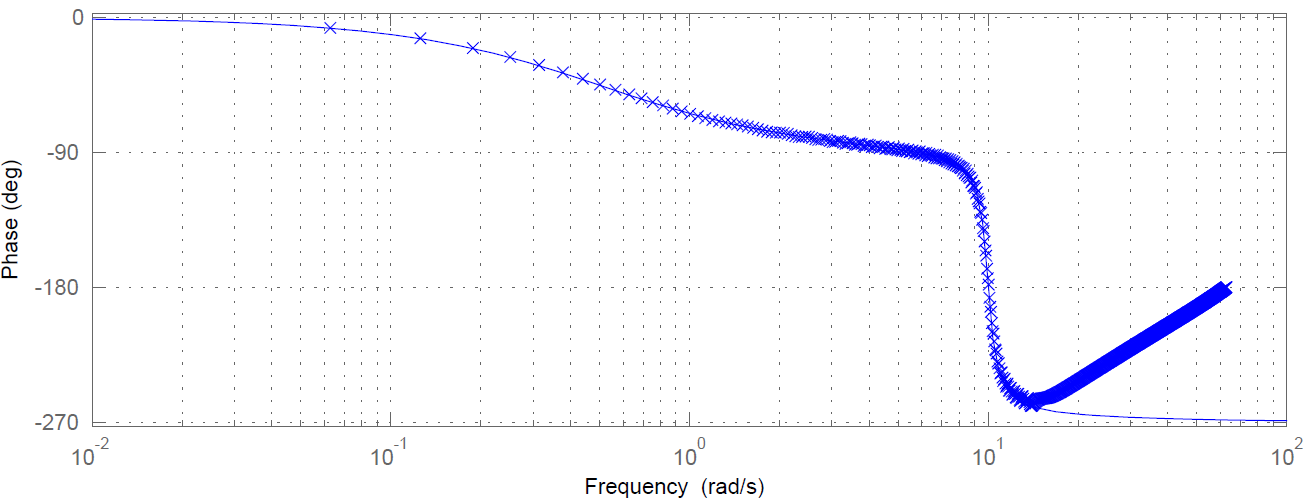
\includegraphics[width=0.3\textwidth]{./bilder/LeakageEffect3.PNG}
	}\\
	\textit{Quelle: Kottmann, Markus (2012): Advanced Control. Introduction to System Idenfication. Version 1.3. 13}
	\label{fig:Leakage}
\end{figure}

\subsubsection{Schrittantwort}
\begin{itemize}
	\item Gibt meist kein ausreichend genaues Modell für die Regelung
	\item Einige Dinge können dennoch mit der Schrittantwort charakterisiert werden, nämlich:
	\begin{itemize}
		\item Statische Verstärkung (DC-Gain)
		\item Dominante Zeitkonstante
		\item Totzeit
		\item Ob das System Resonanzen hat
		\item Minimalphasigkeit des Systems
	\end{itemize}
	\item Schwingt die Schrittantwort zuerst in das Negative, hat das System eine Nullstelle in der rechten Halbebene
	\begin{itemize}
		\item System ist nicht minimalphasig
	\end{itemize}
\end{itemize}

\begin{tabularx}{\linewidth}{p{0.32\linewidth} p{0.32\linewidth} p{0.32\linewidth}}
	\textbf{Nicht minimalphasig}			&\textbf{Totzeit}				&\textbf{PT2}		\\
	%Zeile 2 mit Allen Bildern
	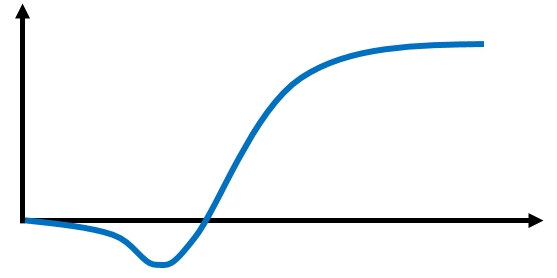
\includegraphics[width=.75\linewidth]{bilder/step1.png}&
	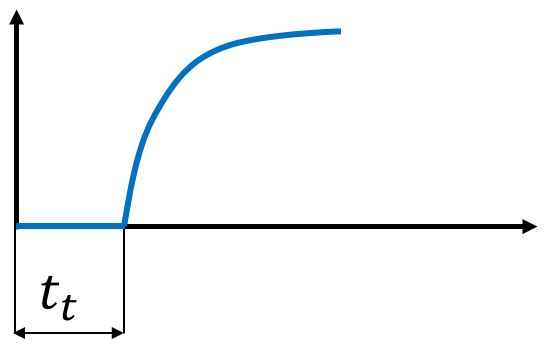
\includegraphics[width=.75\linewidth]{bilder/step2.png}&
	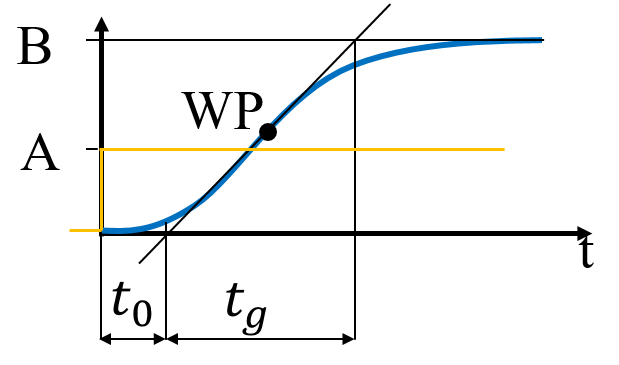
\includegraphics[width=.75\linewidth]{bilder/step3.png} \\
	%Zeile 3 Mit den Formeln
	& \begin{align*}
		G(s)_\text{Totzeit} = e^{-st_t}\\
		G(z)_\text{Totzeit} = z^(-1)
	\end{align*} 
	& \begin{equation*}
	G(s) = \frac{B}{A}\cdot e^{\frac{-s}{T_0}}\cdot \frac{1}{sT_g+1}
	\end{equation*}
\end{tabularx}

\subsection{Parametrische Identifikation}
\begin{itemize}
	\item Identifizieren von Systemen deren Strukturen bekannt sind
	\item Wenn keine Spezielle Form der Systembeschreibung gewählt wird, sind $(n+1)^2$ Parameter zu ermitteln (Matrizen A,B,C,D)
	\begin{itemize}
		\item  Wenn eine spezifische Form gewählt wird (z.B. Regelnormalform) sind es nur noch $2n+1$ Parameter
	\end{itemize}
	\item [1.] Die Matrizen des Systems herleiten (mit den Variablen des Systems, so z.B. Federkonstanten, Dämpfungen, etc.). 
	\item [2.] $G(s)$ aus den Matrizen bestimmen
	\item [3.] Messungen vornehmen und mit den Messergebnissen z.B. Überkoeffizientenvergleich mit $G(s)$ Werte der Parameter bestimmen
\end{itemize}

\subsection{LS-Verfahren}
\begin{itemize}
	\item Fitten von Daten
	\item Es gilt: $N$: Die Anzahl der Datensätze, $n$: Die Anzahl der Variablen
	\item LS zielt darauf ab den Fehler zu minimieren
	\item Verfahren funktioniert besonders gut, wenn gesuchte Funktion Linear in Parameter (im Beispiel $\theta$) ist.
	\begin{itemize}
		\item[] $y_j = f(u_j) = u_j\theta_1+u^2_j\theta_2+\ldots+u^n\theta_n$
		\item $y_j$: Gemessenes Signal, \quad $u_j$: Eingangssignal, \quad $\theta_j$: Parameter
	\end{itemize}
	\item Beispiel (\textit{Quelle: Kottmann, Markus (2012): Advanced Control. Introduction to System Idenfication. Version 1.3. 21}):
	\begin{itemize}
		\item Wenn System überbestimmt ist, braucht es den Fehlerterm $\varepsilon$
		\item Ziel ist es die Kostenfunktion  $J= \vert\varepsilon\vert^2$ klein zu halten (somit also auch $\varepsilon$ klein zu halten)
		\item Mit der gezeigten Formel für $\theta$, wird das $\varepsilon$ bereits minimiert!
	\end{itemize}
\end{itemize}
\begin{align*}
	1. &= 0.8 \theta_1 + 0.8^2\theta_2 = 0.8 \theta_1+0.64\theta_2\\
	2.5 &= 2 \theta_1 + 2^2\theta_2 = 2\theta_1+4\theta_2\\
	2 &= 3 \theta_1 + 3^2\theta_2 = 3 \theta_1+9\theta_2\\
 	\underbrace{ \begin{bmatrix}
 	1 \\ 2.5\\2
 	\end{bmatrix}}_y &= 
	\underbrace{\begin{bmatrix}
		0.8 	& 	0.64\\
		2   	&	4	\\
		3		&	9
		\end{bmatrix}}_\Phi
	\underbrace{\begin{bmatrix}
		\theta_1\\
		\theta_2
		\end{bmatrix}}_\theta\\
	y &= \Phi\theta+\varepsilon\\
	\theta &= \left(\Phi^T\Phi\right)^{-1}\Phi^Ty
\end{align*}

\subsubsection{LS-Verfahren für Zeitdiskrete Systeme}
\begin{itemize}
	\item Vorgehen:
	\begin{itemize}
		\item $G(z)$ umformen, sodass Nenner ein Summand ohne $z$ hat
		\item []$G(z) = \frac{Y(z)}{X(z)} \Leftrightarrow Y(z) = G(z)U(z)$
		\item Parameter (z.B. $a$ und $b$) sind in $G(z)$ enthalten $\Rightarrow$ das ist der Vektor $\theta$
		\item []$  az^{-i}\cdot u(z) \Leftrightarrow au(k-i)$
		\item Umstellen, dass $y(k)$ als Funktion von $y(k-i)$ und $x(k-i)$
		\item $u(k-i)$ und $y(k-i)$ sind die Messwerte am Eingang resp. Ausgang, Versetzt um $i$ Zeitschritte
		\item Daraus erstellen der Matrix $\Phi$ und des Vektors $y$ 
		\item Jeweils eine Zeile je möglicher Gleichung
	\end{itemize}
	\item Siehe auch Kapitel \ref{subsec:LSDynSys}, dort ist die Formel für mehrere Gleichungen angewendet
	\item Minimalbeispiel
\end{itemize}
\begin{align*}
	G(z) &= \frac{Y(z)}{X(z)} = \frac{a}{z\cdot(z+b)}\\
	G(z) &= \frac{az^{-2}}{1+bz^{-1}}\\
	Y(z)\cdot \left(1+bz^{-1}\right) &= X(z)\cdot \left(az^{-2}\right)\\
	Y(z) &= az^{-2}X(z)-bz^{-1}Y(z)\\
	y(k) &= ax(k-2)-by(k-1)\\
	y(k) &= \begin{bmatrix}
		x(k-2) & -y(k-1)
	\end{bmatrix}\begin{bmatrix}
	a \\b
	\end{bmatrix}
\end{align*}

\subsubsection{LS-Verfahren bei Problemen mit Bode-Diagrammen}
\begin{itemize}
	\item Im Komplexen Raum betrachten
	\begin{itemize}
		\item von Amplitudengang und Phasenwinkel zu Polarform
		\item $\vert G(j\omega)\vert=A\left[\text{dB}\right]$ und $\angle G(j\omega) = \varphi \left[\si{\degree}\right] \quad \Rightarrow 10^{A/20}\cdot e^{j\varphi/180}$ 
	\end{itemize}
	\item Minimalbeispiel mit Resonanz und DC-Verstärkung (Gl. = Kommentar zu Gleichung im nachfolgenden Beispiel)
	 \begin{itemize}
	 	\item [Gl.\ref{eq:LS1}:] Normieren, dass Nennerpolynom mit  $s^i$ beginnt
	 	\item [Gl.\ref{eq:LS2}:] Auflösen nach $G(s)s^i$
	 	\item [Gl.\ref{eq:LS3}:] In Frequenzraum wechseln $s\Leftrightarrow(j\omega)$
	 	\item [Gl.\ref{eq:LS4}:] In Matrizen Form bringen (eine Zeile je erhaltenen Messpunkt)
\begin{itemize}
	 	 	\item Nun Werte Einsetzen, dabei wie oben beschrieben Informationen von Bode-Diagramm in Polarform bringen und einsetzen für $G(j\omega)$ 
	 		\item $(j\omega)$ ist $j$ Multpliziert mit der Frequenz an welcher der Messpunkt aufgenommen wurde
\end{itemize}
	 	\item [Gl.\ref{eq:LS5}:] $\tilde{\Phi}$ und $\tilde{y}$ aus dem Real- und Imaginäranteil bilden (Zeilenzahl verdoppelt sich)
	 	\item [Gl.\ref{eq:LS6}:] LS-verfahren so, dass alle Werte am besten gefittet werden. 
	 \end{itemize}
\end{itemize}
\begin{align}
	\label{eq:LS1}
	G(s) &= \frac{k\omega^2}{s^2+2\xi\omega s+\omega^2}\\
	\label{eq:LS2}
	G(s)s^2&=k\omega^2-2G(s)\xi\omega s-G(s)\omega^2\\
	\label{eq:LS3}
	G(j\omega)\left(j\omega\right)^2 &= k\omega^2-2G(j\omega)\xi\omega(j\omega) - G(j\omega)\omega^2\\
	\label{eq:LS4}
	\underbrace{\begin{bmatrix}
		G(j\omega)\left(j\omega\right)^2 
	\end{bmatrix}}_y	&=\underbrace{\begin{bmatrix}
		1	&	-2G(j\omega)(j\omega)	&	-G(j\omega)
	\end{bmatrix}}_\Phi	
	\underbrace{\begin{bmatrix}
		k\omega^2\\
		\xi\omega\\
		\omega^2
	\end{bmatrix}}_\theta\\
	\label{eq:LS5}
	\tilde{y} &= \begin{bmatrix}
		\text{Re}\left(y\right)\\
		\text{Im}\left(y\right)
	\end{bmatrix}	\qquad 
		\tilde{\Phi} = 
	\begin{bmatrix}
		\text{Re}\left(\Phi\right)\\
		\text{Im}\left(\Phi\right)
	\end{bmatrix}\\
	\tilde{y} &= \tilde{\Phi}\theta+\varepsilon\\	
	\label{eq:LS6}
	\theta &= \left(\tilde{\Phi}^T\tilde{\Phi}\right)^{-1}\tilde{\Phi}^T\tilde{y}
\end{align}


\subsubsection{Gewichtetes LS-Verfahren}
\begin{itemize}
	\item Gleichungen haben unterschiedliche Gewichtung (z.B. Arbeitspunkt höher gewichten)
	\begin{itemize}
		\item Gewichtung mit Faktor $\lambda$
		\item Da Gewichtungsmatrix immer als $L^TL$ erscheint, muss für Faktor $\lambda$ stattdessen$\sqrt{\lambda}$ genommen werden
	\end{itemize}
	\item Angewendet auf obige Gleichung ergibt die Auflösung nach $\theta$: 
\end{itemize}
\begin{align*}
	L &= \begin{bmatrix}
		\sqrt{\lambda_1}&0					&\ldots&0\\
		0				&\sqrt{\lambda_2}	&\ldots&0\\
		\vdots			&\vdots				&\ddots&0\\
		0				&0					&\ldots&\sqrt{\lambda_n	}	
	\end{bmatrix}\\
	\theta &= \left(\Phi^TL^TL\Phi\right)^{-1}\Phi^TL^TLy
\end{align*}

\subsubsection{Markov-Annahme unter Verwendung der Co-varianz-Matrix}
\begin{itemize}
	\item $\varepsilon$ ist in Gaussverteilung und der Erwartungswert liegt bei 0
	\item Dann ist die Co-Varianzmatrix: $V= \varepsilon\varepsilon^T$
	\item $\varepsilon$ ist Abweichung zwischen mit dem LS-Verfahren erhaltenem Modell und dem effektiven Messwert
	\item Dann kann für die Gewichtungsfunktion $L^TL=V^{-1}$ genommen werden.
\end{itemize}

\subsection{LS-Verfahren für dynamische Systeme}
\label{subsec:LSDynSys}
\begin{itemize}
	\item Ziel: Ein System welches in Bewegung ist durch zwei Polynome abzubilden
	\item $\varepsilon$ soll möglichst 0 werden
	\item Zwei verschiedene Darstellungsmöglichkeiten für die Modelle (Ausgangsfehlermodell: \ref{subfig:LSNormal}, ARX-Modell: \ref{subfig:LSARX})
\end{itemize}
\begin{figure}[!h]
	\centering
	\subfloat[Ausgangsfehlermodell \label{subfig:LSNormal}]{
		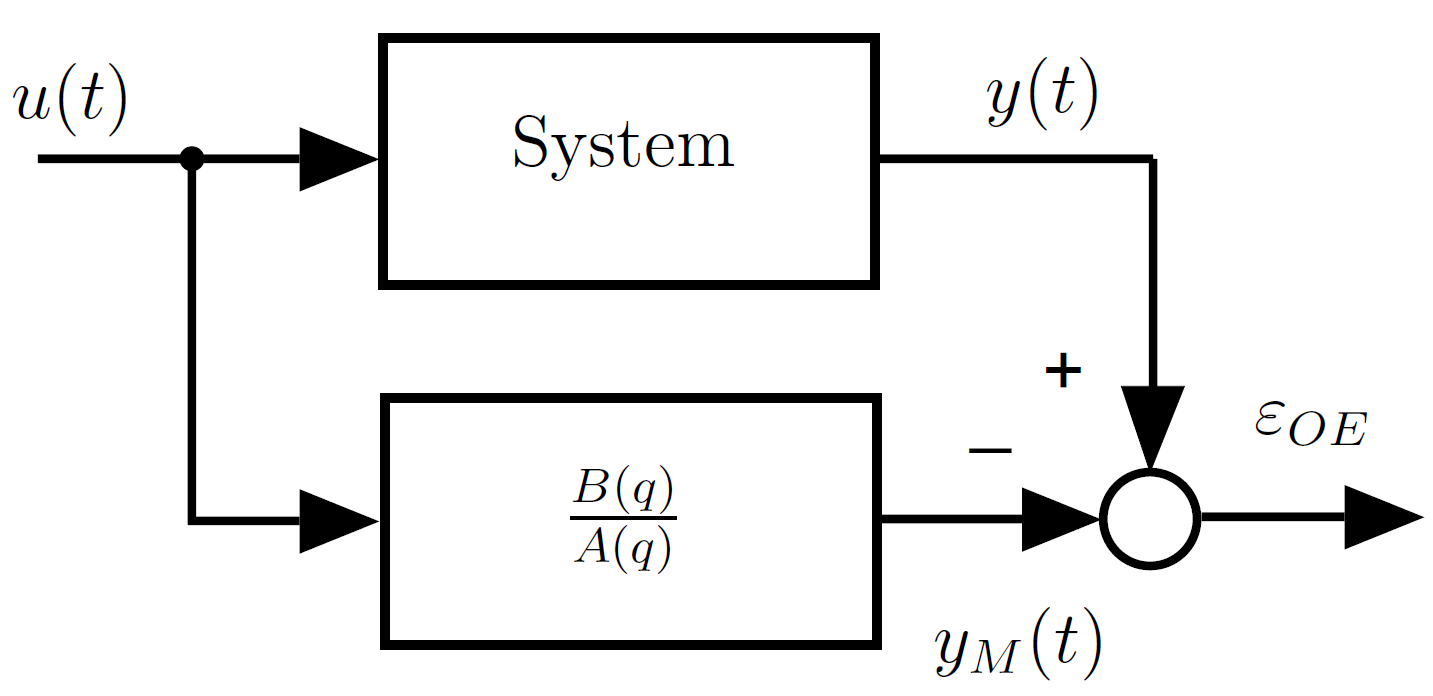
\includegraphics[width=0.3\textwidth]{./bilder/LSNormal.PNG}
	}\hspace{0.1\linewidth} 
	\subfloat[ARX-Modell \label{subfig:LSARX}]{
		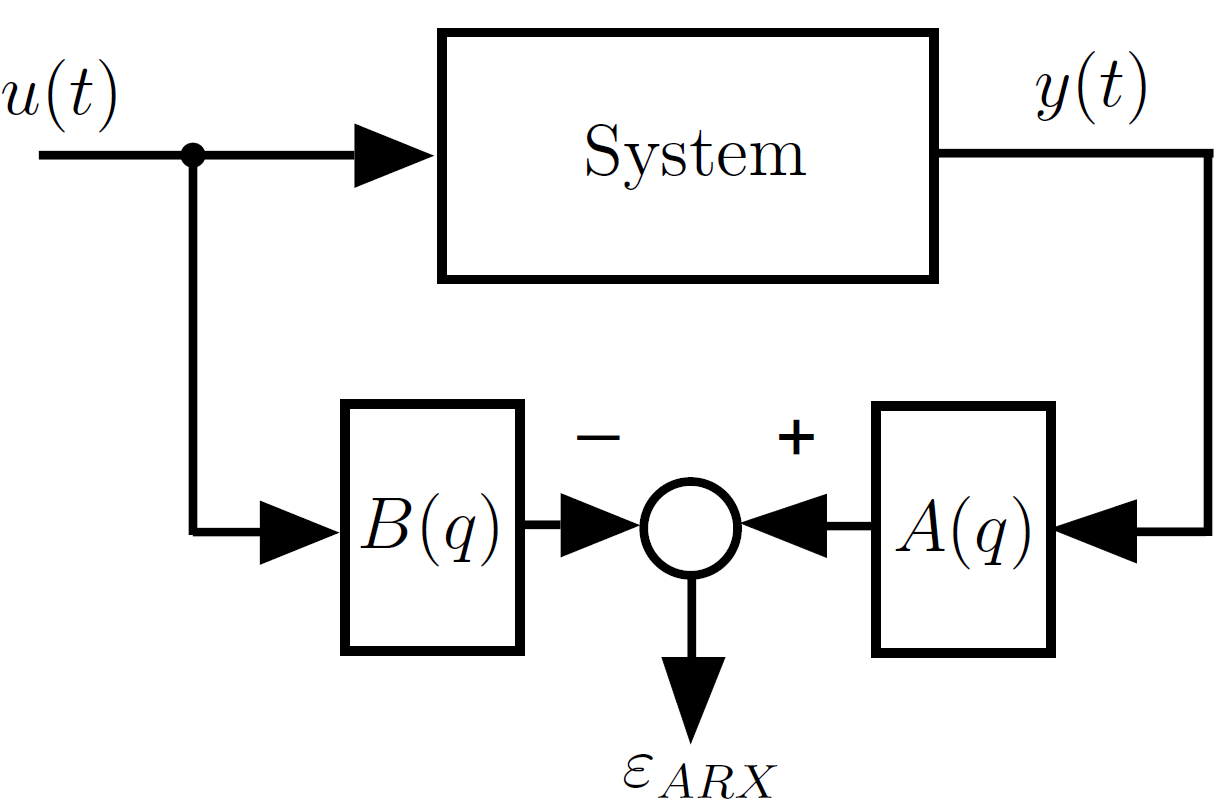
\includegraphics[width=0.25\textwidth]{./bilder/LSARX.PNG}
	}\\
	\caption{Zwei Darstellungsmöglichkeiten für Modelle welche ein LS-Verfahren für dynamische Systeme ermöglichen}
	\textit{Quelle: Kottmann, Markus (2012): Advanced Control. Introduction to System Idenfication. Version 1.3. 26}
	\label{fig:LS}
\end{figure}

\begin{itemize}
	\item Mit der ARX-Struktur kann $y(t)$ angesehn werden als:
	\begin{itemize}
		\item $y(t)$ ist hierbei eine Messung zum Zeitpunkt $k$ und setzt sich aus den vorherigen diskreten Messungen und Eingangssignalen zusammen
	\end{itemize}
\end{itemize}
\begin{align*}
	y(k) 	&= -a_1y(k-1)-\ldots -a_ny(k-n)+b_1u(k-1)+\ldots b_mu(k-m)+\varepsilon(k)\\
			&= \begin{pmatrix}
				-y(k-1) &\ldots &-y(k-n) & u(k-1) & \ldots & u(k-m)
			\end{pmatrix}
			\begin{pmatrix}
				a_1\\ 
				\vdots \\
				a_n\\
				b_1\\
				\vdots\\
				b_m
			\end{pmatrix}+\varepsilon(k)
\end{align*}
\begin{itemize}
	\item Wenn nun $N$ Messungen gemacht werden (somit sind es $0\ldots N$ Messungen)
	\item $\Phi$ sind dabei die am Eingang ($u(k)$ und am Ausgang($y(k)$) gemessenen Signale
	\item Es muss solang gemssen werden, bis $\text{rank}(\Phi) \leq n+m$ (n = Anz. Ausgangssignale, m = Anz. Eingangssignale)
	\item Rekursives LS-Verfahren, siehe Skript s.29
\end{itemize}
\begin{align*}
	\underbrace{\begin{pmatrix}
		y(0)\\
		\vdots\\
		y(N)
	\end{pmatrix}}_y
			&= \underbrace{\begin{pmatrix}
					-y(-1) 	&\ldots 	&-y(-n) 	& u(-1)   	&\ldots 	& u(-m)\\
					\vdots	&\ddots		&\vdots		&\vdots		&\ddots		&\vdots\\	
					-y(N-1) &\ldots 	&-y(N-n) 	& u(N-1) 	&\ldots 	& u(N-m)
					\end{pmatrix}}_{\Phi = \text{Messwerte von Ein- und Ausgnag}}
				\underbrace{\begin{pmatrix}
					a_1\\ 
					\vdots \\
					a_n\\
					b_1\\
					\vdots\\
					b_m
				\end{pmatrix}}_\theta+
				\underbrace{\begin{pmatrix}
					\varepsilon(0)\\
					\vdots\\
					\varepsilon(N)
				\end{pmatrix}}_\varepsilon\\
	\theta	&= \left(\Phi^T\Phi\right)^{-1}\Phi^Ty
\end{align*}
\newpage